%%%%%%%%%%%%%%%%%%%%%%%%%%%%%%%%%%%%%%%%%%%%%%%
%           APPENDIX
%%%%%%%%%%%%%%%%%%%%%%%%%%%%%%%%%%%%%%%%%%%%%%%

% APPENDIX TABLES
\newpage
\section*{Appendix C}
\label{appendix_c}

\setcounter{table}{0}
\renewcommand{\thetable}{C.\arabic{table}} 
\setcounter{figure}{0}
\renewcommand{\thefigure}{C.\arabic{figure}} 

\subsection{Tables}

\begin{table}[!ht]
    \caption{Amount asked (log), amount won (log), and probability of winning - Historic Data}
    \label{Table_Reg_winnings_log}
    \begin{center}

        \scriptsize{% Table generated by Excel2LaTeX from sheet 'TableReg1_log'
\begin{tabular}{lcccc}
\toprule
      & \multicolumn{4}{c}{Panel A : All cases} \\
\midrule
\midrule
      & Total asked & Amount Won & Won/asked & Prob winning \\
\midrule
\midrule
Public Lawyer & -0.62*** & 0.0011 & 0.055** & 1.65 \\
      & (0.033) & (0.22) & (0.024) & (2.33) \\
Constant & 2.76*** & 5.48*** & 1.06*** & 75.6*** \\
      & (0.19) & (0.97) & (0.10) & (9.67) \\
      &       &       &       &  \\
\midrule
Observations & 4866  & 4866  & 4866  & 4866 \\
BVC   & YES   & YES   & YES   & YES \\
Dummy Industry & YES   & YES   & YES   & YES \\
R-squared & 0.74  & 0.036 & 0.043 & 0.020 \\
DepVarMean & 11.7  & 6.40  & 0.21  & 65.3 \\
\midrule
\midrule
      &       &       &       &  \\
\midrule
      & \multicolumn{4}{c}{Panel B : Settlement} \\
\midrule
\midrule
      & Total asked & Amount Won & Won/asked & Prob winning \\
\midrule
\midrule
Public Lawyer & -0.67*** & -0.20*** & 0.087*** & 0.018 \\
      & (0.041) & (0.053) & (0.020) & (0.37) \\
Constant & 2.63*** & 6.59*** & 1.52*** & 99.4*** \\
      & (0.25) & (0.31) & (0.11) & (2.15) \\
      &       &       &       &  \\
\midrule
Observations & 3077  & 3077  & 3077  & 3077 \\
BVC   & YES   & YES   & YES   & YES \\
Dummy Industry & YES   & YES   & YES   & YES \\
R-squared & 0.74  & 0.37  & 0.11  & 0.0068 \\
DepVarMean & 11.7  & 9.70  & 0.27  & 99.6 \\
\midrule
\midrule
      &       &       &       &  \\
\midrule
      & \multicolumn{4}{c}{Panel C: Court ruling} \\
\midrule
\midrule
      & Total asked & Amount Won & Won/asked & Prob winning \\
\midrule
\midrule
Public Lawyer & -0.44*** & -0.22 & 0.027 & -0.59 \\
      & (0.12) & (0.81) & (0.29) & (7.59) \\
Constant & 2.14*** & 0.63  & 1.86** & 7.23 \\
      & (0.68) & (3.14) & (0.84) & (27.5) \\
      &       &       &       &  \\
Observations & 422   & 422   & 422   & 422 \\
BVC   & YES   & YES   & YES   & YES \\
Dummy Industry & YES   & YES   & YES   & YES \\
R-squared & 0.78  & 0.13  & 0.065 & 0.13 \\
DepVarMean & 11.7  & 2.74  & 0.37  & 24.2 \\
\bottomrule
\bottomrule
\end{tabular}%
}
    \end{center}
    \scriptsize
%\begin{figurenotes}
   This table shows OLS regressions of log total amount asked in the initial labor suit, the amount actually won, the ratio of these two, and the probability of the worker recovering a positive amount. Panel A includes all our historical data files (i.e. for all types of case ending), Panel B focuses on cases ending in settlement, and Panel C on those ending in court ruling. All regressions control for our basic variable controls (gender, at will worker, tenure at the firm, daily wage, weekly hours worked), as well as industry dummies in which firm operates in. We have 4866 observations instead of 5005 since there are some missing values in the controls.
     %\textit{Do file: } \texttt{reg_amount.do}
%   \end{figurenotes}     
\end{table}


\begin{table}[!ht]
    \caption{Balance of casefiles having negative recovery amount.}
    \label{negative_returners}
    \begin{center}
    \scriptsize{% Table generated by Excel2LaTeX from sheet 'negative_returners_balance'
\begin{tabular}{lccccc}
\toprule
      & Gender & At will worker & Tenure & Daily wage & Weekly hours \\
\midrule
\midrule
      & (1)   & (2)   & (3)   & (4)   & (5) \\
\midrule
\midrule
Negative NPV & -0.035** & -0.034 & -0.006*** & -0.000 & 0.002*** \\
      & (0.014) & (0.028) & (0.001) & (0.000) & (0.001) \\
Constant & 0.417*** & 0.404*** & 0.428*** & 0.402*** & 0.279*** \\
      & (0.017) & (0.016) & (0.017) & (0.016) & (0.035) \\
      &       &       &       &       &  \\
\midrule
Observations & 4503  & 4492  & 4470  & 4484  & 4425 \\
R-squared & 0.014 & 0.013 & 0.017 & 0.013 & 0.017 \\
F stat & 13.022 & 12.109 & 15.139 & 11.902 & 15.373 \\
Court dummies & YES   & YES   & YES   & YES   & YES \\
\bottomrule
\bottomrule
\end{tabular}%
}
    \end{center}
     \scriptsize
    \textit{Notes:} Each column regresses a characteristic of the case against a dummy variable indicating that the plaintiff recovered an amount less than the MXN\$2000 initial filing fee. The sample is all cases from the historical data using private lawyers.  
         
    %\textit{Do file: } \texttt{negReturnHD.do}
\end{table}


%\begin{table}[!ht]
%   \caption{Treatment description - Phase 1}
%    \label{treatment_description}
%    \begin{center}
%    \scriptsize{\input{paper/Tables/Experiment_description2.tex}}
%    \end{center}
%     \scriptsize
%    \textit{Notes:} This is a short description of the kind of treatment received by each treatment group.
%\end{table}

%\begin{table}[!ht]
%    \caption{Settlements against duration - historical Data}
%    \label{settlement_time}
%    \begin{center}
%    \scriptsize{% Table generated by Excel2LaTeX from sheet 'settlementq_time'
\begin{tabular}{lcccccc}
\toprule
      & \multicolumn{2}{c}{Settlement amount} & \multicolumn{2}{c}{Settlement amt discounted} & \multicolumn{2}{c}{Calculator prediction} \\
\midrule
\midrule
      & (1)   & (2)   & (3)   & (4)   & (5)   & (6) \\
\midrule
\midrule
Months  & 1202.9*** &       & -166.3** &       & 180.0*** &  \\
      & (166.8) &       & (70.37) &       & (30.82) &  \\
2 Quintil &       & 4052.7** &       & 1754.3 &       & 1576.3*** \\
      &       & (1859.3) &       & (1676.1) &       & (460.2) \\
3 Quintil &       & 1622.4 &       & -1767.8 &       & 1451.0** \\
      &       & (2015.3) &       & (1705.6) &       & (565.7) \\
4 Quintil &       & 8663.2*** &       & 44.58 &       & 3029.1*** \\
      &       & (2348.7) &       & (1808.5) &       & (595.2) \\
5 Quintil &       & 21982.6*** &       & -3474.0* &       & 3990.9*** \\
      &       & (3299.9) &       & (1882.0) &       & (718.8) \\
Constant  & 10907.8*** & 15396.9*** & 15841.8*** & 14649.2*** & 9544.0*** & 9331.9*** \\
      & (4229.2) & (4326.9) & (2953.9) & (3018.0) & (1031.9) & (1076.7) \\
      &       &       &       &       &       &  \\
\midrule
Observations  & 3080  & 3080  & 3080  & 3080  & 3081  & 3081 \\
R-squared & 0.24  & 0.23  & 0.22  & 0.22  & 0.66  & 0.65 \\
BVC   & YES   & YES   & YES   & YES   & YES   & YES \\
\bottomrule
\bottomrule
\end{tabular}%
}
%    \end{center}
%     \scriptsize
%    \textit{Notes:} 
%    This table focuses on the sample of cases from the historical data (HD) that settled at any point in time (3080 cases out of 5005). Each column is a different regression. All regressions control for the basic variables of the case (BVC) which are described in Panel B of Table 1. Columns 1 and 2 have as a dependent variable the settlement amount in pesos the worker actually got in the settlement. Column 1 regresses this amount on a counter for the number of months that elapsed from the initial filing until the settlement. Column 2 breaks this elapsed time in quintiles dummies. Columns 3 and 4 discount the peso amount at a 3.43 monthly rate. This rate was calculated by matching our sample to that of the MxFls survey and obtaining the elicited time discount rate for similar individuals (using gender, age, education, daily wage, and weekly hours), and taking the median. Columns 5 and 6 use the prediction from our ``calculator'', that is, the amount they would get on average given the initial case characteristics, with no discounting.
    %\textit{Do file: } \texttt{settlementq\_time.do}
%\end{table}

\begin{table}[!ht]
    \caption{Balance regression on characteristics conditional on employee present}
    \label{ep_balance}
    \begin{center}
    \scriptsize{% Table generated by Excel2LaTeX from sheet 'ep_balance'
\begin{tabular}{rccccc}
\toprule
      & Control & Calculator & Observations & R-squared & p-value (calculator = 0) \\
\midrule
\midrule
\multicolumn{1}{l}{Public Lawyer} & 0.223*** & 0.034 & 312   & 0.042 & 0.492 \\
      & (0.043) & (0.049) &       &       &  \\
\multicolumn{1}{l}{Gender} & 0.162* & -0.256** & 312   & 0.080 & 0.0395 \\
      & (0.0890) & (0.121) &       &       &  \\
\multicolumn{1}{l}{At will worker} & 0.0197 & -0.0351 & 312   & 0.049 & 0.742 \\
      & (0.0965) & (0.106) &       &       &  \\
\multicolumn{1}{l}{Tenure} & 0.189 & -0.286* & 306   & 0.068 & 0.0814 \\
      & (0.133) & (0.161) & .     &       &  \\
\multicolumn{1}{l}{Daily wage} & 0.0659 & -0.0975 & 307   & 0.006 & 0.493 \\
      & (0.141) & (0.141) &       &       &  \\
\multicolumn{1}{l}{Weekly hours} & 0.0230 & -0.0203 & 306   & 0.136 & 0.863 \\
      & (0.0755) & (0.117) &       &       &  \\
\bottomrule
\bottomrule
\end{tabular}%
}
    \end{center}
     \scriptsize
    \textit{Notes:} The table shows results of regressions with the specification $y_i = \alpha_t + \beta T_i + \epsilon_{i}$. The sample is limited to the cases in which the plaintiff was present at the hearing.  Each columns represents a different regression with the indicated independent variable. The regressions all include subcourt fixed effects. 
         
    %\textit{Do file: } \texttt{ep\_balance.do}
\end{table}




\begin{table}[!ht]
    \caption{Employee presence}
    \label{pactor_reg}
    \begin{center}
    \scriptsize{% Table generated by Excel2LaTeX from sheet 'pactor_reg'
\begin{tabular}{lccc}
\toprule
      & \multicolumn{3}{c}{Employee Present} \\
\midrule
\midrule
      & Phase 1 & Phase 2 & Phase 1/2 \\
\midrule
\midrule
      & (1)   & (2)   & (3) \\
\midrule
\midrule
Female & -0.066* & 0.000 & -0.023 \\
      & (0.035) & (0.023) & (0.019) \\
Public Lawyer & 0.317*** & 0.508*** & 0.416*** \\
      & (0.066) & (0.059) & (0.045) \\
At will worker & -0.063 & 0.013 & -0.016 \\
      & (0.049) & (0.042) & (0.032) \\
Tenure (years) & 0.004 & 0.005** & 0.005*** \\
      & (0.003) & (0.002) & (0.002) \\
Daily wage & -0.000 & -0.000 & -0.000 \\
      & (0.000) & (0.000) & (0.000) \\
Weeky hours & -0.002** & -0.003*** & -0.003*** \\
      & (0.001) & (0.001) & (0.001) \\
Age   &       & -0.001 &  \\
      &       & (0.003) &  \\
Constant & 0.313*** & 0.303*** & 0.298*** \\
      & (0.062) & (0.066) & (0.045) \\
      &       &       &  \\
\midrule
Observations & 520   & 1026  & 1546 \\
R-squared & 0.090 & 0.124 & 0.105 \\
DepVarMean & 0.208 & 0.183 & 0.191 \\
p-value & 0.000 & 0.000 & 0.000 \\
p-value w/o PL & 0.014 & 0.001 & 0.000 \\
\bottomrule
\bottomrule
\end{tabular}%
}
    \end{center}
    \scriptsize
    \textit{Notes:} OLS of employee presence against basic variable controls as predictors. Last two rows shows the p-value testing the quality of all basic variables ( \& without public lawyer) respectively.
     
    % \textit{Do file: } \texttt{pEmployeePresence.do}
\end{table}

\begin{table}[!ht]
    \caption{Expectations Relative to Prediction}
    \label{prediction_cases}
   % \scriptsize{% Table generated by Excel2LaTeX from sheet 'prediction_cases_pooled'
\begin{tabular}{lcccc}
\toprule
      & \multicolumn{2}{c}{Expectation} & \multicolumn{2}{c}{Relative OC} \\
\midrule
\midrule
      & Probability & Amount & Probability & Amount \\
\midrule
      & (1)   & (2)   & (3)   & (4) \\
\midrule
\midrule
Employee's Lawyer & 4.52  & 5902.2 & 0.22  & -0.097 \\
      & (3.46) & (12555.8) & (0.14) & (0.53) \\
Firm's Lawyer & -27.4*** & -27573.0** & -0.96*** & -0.38 \\
      & (3.34) & (12083.0) & (0.13) & (0.50) \\
Constant & 75.0*** & 74788.7*** & 1.64*** & 0.73* \\
      & (2.86) & (10219.5) & (0.11) & (0.43) \\
      &       &       &       &  \\
\midrule
Observations & 2214  & 1859  & 1952  & 1632 \\
File Fixed Effects & YES   & YES   & YES   & YES \\
R-squared & 0.83  & 0.89  & 0.96  & 0.89 \\
p-value:Emp Law & 0     & 0     & 0     & 0 \\
p-value:Firm Law & 0     & 0     & 0     & 0.1 \\
\bottomrule
\bottomrule
\end{tabular}%
}
   \begin{center}
    \scriptsize{% Table generated by Excel2LaTeX from sheet 'prediction_cases_pooled_panels'
\begin{tabular}{lccccc}
\toprule
\multicolumn{6}{c}{\textbf{Panel A}} \\
\midrule
      & \multicolumn{2}{c}{Expectation} &       & \multicolumn{2}{c}{Relative OC} \\
\cmidrule{2-3}\cmidrule{5-6}      & Probability & Amount &       & Probability & Amount \\
\midrule
      & (1)   & (2)   &       & (3)   & (4) \\
\midrule
\midrule
Employee's Lawyer ($\beta_1$) & 0.070 & 11410.9 &       & 0.28  & -0.17 \\
      & (0.044) & (13314.9) &       & (0.18) & (0.71) \\
Firm's Lawyer ($\beta_2$) & -0.25*** & -21804.2* &       & -0.86*** & -0.51 \\
      & (0.042) & (12614.9) &       & (0.17) & (0.67) \\
Constant (employee $\alpha$) & 0.74*** & 66755.3*** &       & 1.70*** & 1.00* \\
      & (0.036) & (10791.5) &       & (0.15) & (0.58) \\
      &       &       &       &       &  \\
\midrule
Observations & 1274  & 1104  &       & 1177  & 1032 \\
File Fixed Effects & YES   & YES   &       & YES   & YES \\
R-squared & 0.79  & 0.91  &       & 0.96  & 0.89 \\
p-value:Emp Law & 0     & 0     &       & 0     & 0 \\
p-value:Firm Law & 0     & 0     &       & 0     & 0.04 \\
\midrule
\midrule
      &       &       &       &       &  \\
\midrule
\multicolumn{6}{c}{\textbf{Panel B}} \\
\midrule
      & \multicolumn{2}{c}{Expectation} &       & \multicolumn{2}{c}{Relative OC} \\
\cmidrule{2-3}\cmidrule{5-6}      & Probability & Amount &       & \multicolumn{2}{c}{Amount} \\
\midrule
      & (1)   & (2)   &       & (3)   & (4) \\
\midrule
\midrule
Mean  & 0.885*** & 58,077*** &       & 1.713*** & 1.315*** \\
      & (0.00288) & (1,794) &       & (0.0729) & (0.0619) \\
Standar deviation & 0.166 & 74471 &       & 3.026 & 2.570 \\
      &       &       &       &       &  \\
\midrule
Observations & 3,330 & 1,723 &       & 1,723 & 1,723 \\
Ignores prob. (\%) & 13.08 &       &       &       &  \\
Standard deviation & 0.166 & 74471 &       & 3.026 & 2.570 \\
Reference &       &       &       & Mid prediction & Max prediction \\
\bottomrule
\bottomrule
\end{tabular}%
}
    \end{center}
% \begin{figurenotes}
    \scriptsize
\textit{Notes:} The table regresses measures of expectation elicited in the baseline survey on dummies of who is the respondent of the survey. For some cases we could elicit the expectation of more than one party (employee, employee's lawyer, firm's lawyer). The omitted variable is the employee dummy, so the interpretation of the employee's lawyer and firm's lawyer coefficients are relative to the employee who is captured in the constant. It combines two phases in one singled pooled dataset. Each column represents a different regression. The first column use elicited probability of winning as a dependent variable. The exact question is: \textit{``How likely is it that you will win the lawsuit if it ends in a court judgment?''}. The second column use the peso amount (undiscounted) that they expect to recover conditional on winning. The exact wording of the survey question is: \textit{``in case you win the lawsuit, what amount are you most likely to win?''}.  All columns include casefile fixed effects, avoiding the comparison across casefiles. The bottom of the table present the p-values of two null hypothesis:  $\alpha + \beta_1=0$, and $\alpha + \beta_2=0$, telling us whether the employee's lawyer, or firm's lawyer are more or less confident. Last 2 columns use a measure of ``overconfidence'', which compares the subjective expectation vs the personalized calculator prediction. Relative OC is computed as $\frac{expectation-prediction}{prediction}$, where expectation refers to the expectation measured in the baseline survey.
    %\textit{Do file: } \texttt{prediction\_cases\_pooled.do, ExpectationsFromP3forPrediction_cases_pooles_panelB.do}
 %  \end{figurenotes}    
\end{table}

%Old version of other PSM tabel?
%\begin{table}[!ht]
%    \caption{Comparison of settlement amounts}
%    \label{match_table_lr}
%     \begin{center}
%      \centering
%        \scriptsize{% Table generated by Excel2LaTeX from sheet 'NN_match_lr'
\begin{tabular}{lcccc|cc}
\toprule
\multicolumn{7}{c}{Treatment effect. Nearest-neighbor matching} \\
\midrule
\midrule
      & \multicolumn{6}{c}{Phase 1/2} \\
\midrule
\midrule
      & \multicolumn{4}{c|}{Variable matching} & \multicolumn{2}{c}{PSM} \\
\midrule
\midrule
      & (1)   & (2)   & (3)   & (4)   & (5)   & (6) \\
\midrule
ATE   & 6154  & 8867** & 6893* & 9852** & 8079* & 11829** \\
      & (5303) & (4302) & (5310) & (4328) & (6691) & (5345) \\
\% ATE & 81    & 116   & 90    & 129   & 106   & 155 \\
Baseline mean & \multicolumn{6}{c}{7622} \\
Obs   & \multicolumn{6}{c}{89} \\
Obs HD & \multicolumn{6}{c}{414} \\
Bias adjustment & NO    & NO    & YES   & YES   & -     & - \\
Matches & [1-1] & [1-3] & [1-1] & [1-3] & [1-1] & [1-3] \\
\bottomrule
\bottomrule
\end{tabular}%
}
%    \end{center}%
%  \scriptsize
%    \textit{Notes:}
 %  This table is a robustness check considering all cases settled up to December 2018, contrary to cases settled on the same day as Table \ref{match_table}.  See the notes to \ref{match_table} for further details. 
 
   %\textit{Do file: } \texttt{settlement\_conciliator\_matching\_lr.do}
%\end{table}

\begin{table}[!ht]
    \caption{First stage and robustness for the control function regression}
    \label{table_fs_cf}
    \begin{center}
    \scriptsize{% Table generated by Excel2LaTeX from sheet 'fs_treatment_effects'
\begin{tabular}{lcccccccccc}
\toprule
      & \multicolumn{7}{c}{Settlement}                        &       & \multicolumn{2}{c}{Emp present} \\
\cmidrule{2-8}\cmidrule{10-11}      & Probit &       & \multicolumn{2}{c}{OLS} &       & \multicolumn{2}{c}{Probit} &       & OLS   & Probit \\
\cmidrule{2-2}\cmidrule{4-5}\cmidrule{7-8}\cmidrule{10-11}      & (1)   &       & (2)   & (3)   &       & (4)   & (5)   &       & (6)   & (7) \\
\midrule
\midrule
Calculator  & 0.121 &       &       &       &       &       &       &       & 0.0288 & 0.108 \\
      & (0.0950) &       &       &       &       &       &       &       & (0.0175) & (0.0680) \\
Emp present (EP) & 0.723*** &       &       &       &       &       &       &       &       &  \\
      & (0.163) &       &       &       &       &       &       &       &       &  \\
Calculator\#EP & 0.257 &       &       &       &       &       &       &       &       &  \\
      & (0.189) &       &       &       &       &       &       &       &       &  \\
\multicolumn{1}{r}{9:30} &       &       & -0.0496 & -0.0397 &       & -0.218 & -0.213 &       & -0.0410 & -0.133 \\
      &       &       & (0.0410) & (0.0389) &       & (0.168) & (0.227) &       & (0.0401) & (0.138) \\
\multicolumn{1}{r}{10:00} &       &       & -0.0604* & -0.0130 &       & -0.279** & -0.0755 &       & -0.0878*** & -0.326*** \\
      &       &       & (0.0312) & (0.0295) &       & (0.135) & (0.167) &       & (0.0317) & (0.115) \\
\multicolumn{1}{r}{10:30} &       &       & -0.0471 & -0.0423 &       & -0.226 & -0.272 &       & -0.0474 & -0.157 \\
      &       &       & (0.0398) & (0.0389) &       & (0.159) & (0.220) &       & (0.0376) & (0.131) \\
\multicolumn{1}{r}{11:00} &       &       & -0.0744** & -0.0311 &       & -0.354** & -0.189 &       & -0.0649* & -0.224* \\
      &       &       & (0.0321) & (0.0298) &       & (0.141) & (0.172) &       & (0.0334) & (0.121) \\
\multicolumn{1}{r}{11:30} &       &       & -0.0904** & -0.0440 &       & -0.412** & -0.264 &       & -0.129*** & -0.503*** \\
      &       &       & (0.0414) & (0.0417) &       & (0.176) & (0.218) &       & (0.0406) & (0.174) \\
\multicolumn{1}{r}{12:00} &       &       & -0.0648* & -0.0248 &       & -0.301** & -0.182 &       & -0.0419 & -0.138 \\
      &       &       & (0.0373) & (0.0380) &       & (0.152) & (0.201) &       & (0.0353) & (0.119) \\
\multicolumn{1}{r}{12:30} &       &       & 0.306** & 0.293* &       & 0.672* & 0.654 &       & -0.0142 & -0.0297 \\
      &       &       & (0.137) & (0.155) &       & (0.395) & (0.427) &       & (0.122) & (0.435) \\
      &       &       &       &       &       &       &       &       &       &  \\
\midrule
Observations & 1700  &       & 1723  & 1401  &       & 1700  & 1348  &       & 1732  & 1732 \\
R-squared & 0.149 &       & 0.080 & 0.101 &       & 0.0870 & 0.119 &       & 0.037 & 0.0427 \\
Control Mean & \multicolumn{7}{c}{0.116}                             &       & \multicolumn{2}{c}{0.174} \\
$H_0 : Z=0$ (p-value) &       &       & 0.0323 & 0.191 &       & 0.0331 & 0.202 &       & 0.0670 & 0.0844 \\
Conditional on EP=0 &       &       &       & \checkmark &       &       & \checkmark &       &       &  \\
\bottomrule
\bottomrule
\end{tabular}%
}
    \end{center}
     \scriptsize
    \textit{Notes:} The first column repeats the regression in column 5 of \ref{Treatment_effects} using a probit specification rather than a linear probability model. Column (2) is a `reduced form' OLS regression, and column (3) conditions on employee \emph{not} being present. This serves as a test that time of the hearing does not affect settlement for reasons other than the plaintiff's presence. In the bottom panel we included the p-value for the null that the instrumental variables are equal to zero. Columns (4)-(5) are analogous to columns(2)-(3) but with a probit specification. The sixth column is a OLS first stage for employee present, and column (7) is the probit FS used in the control function of table \ref{Treatment_effects}. See the notes to \ref{Treatment_effects} for further details. 
         
    %\textit{Do file: } \texttt{fs_treatment_effects.do}
\end{table}

% \begin{table}[!ht]
%     \caption{Presence of each party at time of hearing}
%     \label{table_fs_cf}
%     \begin{center}
%     \scriptsize{% Table generated by Excel2LaTeX from sheet 'presence_time_hearing'
\begin{tabular}{lccc}
\toprule
      & Emp present & Employee's Lawyer & Defendant \\
\midrule
      & (1)   & (2)   & (3) \\
\midrule
\midrule
\multicolumn{1}{r}{9:30} & -0.0387 & -0.0438 & -0.0236 \\
      & (0.0400) & (0.0352) & (0.0356) \\
\multicolumn{1}{r}{10:00} & -0.0877*** & 0.00589 & -0.0555 \\
      & (0.0329) & (0.0254) & (0.0347) \\
\multicolumn{1}{r}{10:30} & -0.0503 & -0.0146 & -0.0692* \\
      & (0.0373) & (0.0317) & (0.0406) \\
\multicolumn{1}{r}{11:00} & -0.0677* & -0.0177 & -0.0730** \\
      & (0.0346) & (0.0282) & (0.0371) \\
\multicolumn{1}{r}{11:30} & -0.128*** & -0.0374 & -0.0789 \\
      & (0.0402) & (0.0387) & (0.0487) \\
\multicolumn{1}{r}{12:00} & -0.0279 & 0.00838 & -0.150*** \\
      & (0.0358) & (0.0281) & (0.0419) \\
\multicolumn{1}{r}{12:30} & -0.0433 & 0.114*** & -0.0365 \\
      & (0.121) & (0.0195) & (0.136) \\
Constant (9:00) & 0.243*** & 0.886*** & 0.837*** \\
      & (0.0275) & (0.0195) & (0.0235) \\
      &       &       &  \\
\midrule
Observations & 1732  & 1732  & 1732 \\
R-squared & 0.009 & 0.004 & 0.011 \\
DepVarMean & 0.186 & 0.876 & 0.773 \\
F p-value & 0.0614 & 1.49e-35 & 0.0487 \\
\bottomrule
\bottomrule
\end{tabular}%
}
%     \end{center}
%      \scriptsize
%     \textit{Notes:} This table shows the correlation between attendance to hearing of each party involved and the time of hearing.
         
%     %\textit{Do file: } \texttt{presence\_time\_hearing.do}
% \end{table}



\begin{table}[!ht]
    \caption{Time of hearing balance table}
    \label{pactor_balance}
    \begin{center}
    \scriptsize{% Table generated by Excel2LaTeX from sheet 'balance_instrument'
\begin{tabular}{lcccccc}
\toprule
      & Tenure & Public Lawyer & \% severance pay & Daily wage & \% tenure bonus & Entitlement \\
\midrule
      & (1)   & (2)   & (3)   & (4)   & (5)   & (6) \\
\midrule
\midrule
\multicolumn{1}{r}{9:30} & -0.346 & 0.0145 & -0.0666* & 6.814 & -0.0151 & 8909.1 \\
      & (0.623) & (0.0228) & (0.0391) & (91.44) & (0.0428) & (10278.3) \\
\multicolumn{1}{r}{10:00} & -0.648 & 0.0374* & -0.0600** & 81.40 & -0.0328 & 11390.7 \\
      & (0.445) & (0.0204) & (0.0298) & (92.32) & (0.0318) & (9100.5) \\
\multicolumn{1}{r}{10:30} & -0.596 & 0.0325 & -0.00204 & -13.54 & 0.0265 & 1243.9 \\
      & (0.498) & (0.0244) & (0.0370) & (88.12) & (0.0342) & (8802.9) \\
\multicolumn{1}{r}{11:00} & -0.382 & 0.0235 & -0.0613* & 146.9 & -0.0439 & 16760.3 \\
      & (0.491) & (0.0214) & (0.0363) & (109.7) & (0.0367) & (10639.8) \\
\multicolumn{1}{r}{11:30} & -0.759 & 0.00113 & -0.0702 & -36.98 & -0.0501 & -3711.1 \\
      & (0.507) & (0.0223) & (0.0453) & (118.4) & (0.0479) & (11996.4) \\
\multicolumn{1}{r}{12:00} & -0.531 & 0.0522** & -0.0637 & -61.97 & -0.0163 & -4735.1 \\
      & (0.582) & (0.0249) & (0.0389) & (75.50) & (0.0369) & (7210.8) \\
\multicolumn{1}{r}{12:30} & -0.0313 & -0.0551*** & -0.158 & -164.6 & -0.219* & -12849.4 \\
      & (1.148) & (0.0145) & (0.139) & (149.1) & (0.122) & (14470.0) \\
Constant (9:00) & 4.920*** & 0.0551*** & 0.858*** & 627.0*** & 0.819*** & 67822.2*** \\
      & (0.358) & (0.0145) & (0.0229) & (57.20) & (0.0247) & (5456.1) \\
      &       &       &       &       &       &  \\
\midrule
Observations & 1585  & 1635  & 1634  & 1613  & 1635  & 1617 \\
R-squared & 0.002 & 0.005 & 0.006 & 0.004 & 0.005 & 0.004 \\
F p-value & 0.741 & 1.06e-18 & 0.240 & 0.455 & 0.123 & 0.323 \\
\bottomrule
\bottomrule
\end{tabular}%
}
    \end{center}
    \scriptsize
    \textit{Notes:} This table assess balance in covariates for the distinct times of hearing, which is the variable we use as instrument for employee presence in the control function.
     
    % \textit{Do file: } \texttt{balance_instrument.do}
\end{table}


%Commented table
\begin{comment}
\begin{table}[!ht]
    \caption{Treatment Effects with different end mode outcomes}
    \label{te_end_mode}
    \begin{center}
    \scriptsize{% Table generated by Excel2LaTeX from sheet 'treatment_effects_end_mode'
\begin{tabular}{lcccc}
\toprule
      & \multicolumn{4}{c}{Phase 1/2 (Long run)} \\
\midrule
      & Settlement & \multicolumn{1}{p{4.835em}}{Court ruling\newline{}w/ payment} & \multicolumn{1}{p{4.055em}}{Court ruling\newline{}w/o payment} & Drop / Settle \\
\midrule
\midrule
      & (1)   & (2)   & (3)   & (4) \\
\midrule
\midrule
Control (constant) & 0.47*** & 0.083*** & 0.14*** & 0.20*** \\
      & (0.045) & (0.023) & (0.034) & (0.035) \\
Calculator & 0.0025 & -0.0030 & -0.022 & 0.0073 \\
      & (0.025) & (0.013) & (0.029) & (0.022) \\
Emp present (EP) & 0.072 & 0.010 & -0.077* & 0.041 \\
      & (0.051) & (0.031) & (0.043) & (0.041) \\
Calculator\#EP & 0.12* & -0.016 & -0.010 & -0.072 \\
      & (0.066) & (0.036) & (0.052) & (0.046) \\
      &       &       &       &  \\
\midrule
Observations & 1726  & 1726  & 1726  & 1726 \\
R-squared & 0.082 & 0.0047 & 0.13  & 0.012 \\
Court dummies  & YES   & YES   & YES   & YES \\
DepVarMean & 0.45  & 0.059 & 0.22  & 0.14 \\
IntVarMean & 0.56  & 0.059 & 0.17  & 0.13 \\
\bottomrule
\bottomrule
\end{tabular}%
}
    \end{center}
     \scriptsize
    \textit{Notes:} 
         This table indicates the treatment effects for both experimental phases taking different type of ending outcomes. See the notes to \ref{Treatment_effects} for further details.
    %\textit{Do file: } \texttt{treatment\_effects\_end_\mode.do }
\end{table}
\end{comment}

\begin{table}[!ht]
    \caption{Heterogeneity in treatment effects}
    \label{te_heterogeneity}
    \begin{center}
    \scriptsize{% Table generated by Excel2LaTeX from sheet 'te_heterogeneity'
\begin{tabular}{lccccccccc}
\toprule
Interaction var & \multicolumn{3}{c}{Daily wage} & \multicolumn{3}{c}{Tenure} & \multicolumn{3}{c}{Weekly hours} \\
\midrule
\midrule
      & Phase 1 & Phase 2 & Phase 1/2 & Phase 1 & Phase 2 & Phase 1/2 & Phase 1 & Phase 2 & Phase 1/2 \\
\midrule
      & (1)   & (2)   & (3)   & (4)   & (5)   & (6)   & (7)   & (8)   & (9) \\
\midrule
\midrule
Control (Constant) & 0.051*** & 0.076 & 0.081** & 0.051*** & 0.096** & 0.069* & 0.069*** & 0.10** & 0.10*** \\
      & (0.017) & (0.045) & (0.035) & (0.018) & (0.042) & (0.036) & (0.022) & (0.044) & (0.032) \\
Calculator & 0.090** & 0.041 & 0.00091 & 0.080** & 0.042* & 0.014 & 0.053 & 0.027 & 0.0022 \\
      & (0.039) & (0.027) & (0.019) & (0.036) & (0.021) & (0.020) & (0.043) & (0.038) & (0.026) \\
Interaction Var (Int) & 0.049 & 0.084 & 0.037 & 0.042 & 0.047 & 0.056** & 0.012 & 0.017 & -0.022 \\
      & (0.032) & (0.060) & (0.038) & (0.030) & (0.041) & (0.027) & (0.032) & (0.044) & (0.024) \\
Calculator\#Int & -0.073 & 0.0028 & 0.027 & -0.062 & -0.011 & -0.00026 & 0.0054 & 0.033 & 0.026 \\
      & (0.060) & (0.065) & (0.044) & (0.055) & (0.043) & (0.032) & (0.056) & (0.063) & (0.041) \\
Emp present (EP) &       &       & 0.047 &       &       & 0.16*** &       &       & 0.024 \\
      &       &       & (0.050) &       &       & (0.050) &       &       & (0.072) \\
Calculator\#EP   &       &       & 0.30*** &       &       & 0.21*** &       &       & 0.26*** \\
      &       &       & (0.078) &       &       & (0.067) &       &       & (0.093) \\
EP\#Int &       &       & 0.15* &       &       & 0.0045 &       &       & 0.16 \\
      &       &       & (0.078) &       &       & (0.074) &       &       & (0.096) \\
Calculator\#EP\#Int &       &       & -0.24** &       &       & -0.13 &       &       & -0.13 \\
      &       &       & (0.10) &       &       & (0.093) &       &       & (0.13) \\
      &       &       &       &       &       &       &       &       &  \\
\midrule
Observations & 540   & 1073  & 1613  & 538   & 1047  & 1585  & 536   & 1080  & 1616 \\
R-squared & 0.013 & 0.060 & 0.13  & 0.010 & 0.053 & 0.14  & 0.0090 & 0.053 & 0.13 \\
DepVarMean & 0.10  & 0.21  &       & 0.097 & 0.21  &       & 0.10  & 0.20  &  \\
\midrule
\midrule
      &       &       &       &       &       &       &       &       &  \\
\midrule
Interaction var & \multicolumn{3}{c}{Gender} & \multicolumn{3}{c}{Public Lawyer} & \multicolumn{3}{c}{Entitlement} \\
\midrule
\midrule
      & Phase 1 & Phase 2 & Phase 1/2 & Phase 1 & Phase 2 & Phase 1/2 & Phase 1 & Phase 2 & Phase 1/2 \\
\midrule
      & (10)  & (11)  & (12)  & (13)  & (14)  & (15)  & (16)  & (17)  & (18) \\
\midrule
\midrule
Control (Constant) & 0.075*** & 0.084* & 0.087*** & 0.064*** & 0.11*** & 0.096*** & 0.053*** & 0.055 & 0.066* \\
      & (0.021) & (0.043) & (0.031) & (0.016) & (0.028) & (0.027) & (0.020) & (0.042) & (0.034) \\
Calculator & 0.074* & 0.068** & 0.012 & 0.055* & 0.043* & 0.014 & 0.066* & 0.057* & 0.0033 \\
      & (0.038) & (0.025) & (0.018) & (0.029) & (0.023) & (0.016) & (0.036) & (0.029) & (0.019) \\
Interaction Var (Int) & -0.0017 & 0.067 & 0.023 & 0.092 & 0.041 & -0.027 & 0.039 & 0.11** & 0.064* \\
      & (0.034) & (0.043) & (0.023) & (0.059) & (0.11) & (0.041) & (0.033) & (0.049) & (0.035) \\
Calculator\#Int & -0.053 & -0.052 & 0.0068 & -0.030 & -0.030 & 0.0034 & -0.027 & -0.020 & 0.021 \\
      & (0.059) & (0.040) & (0.027) & (0.082) & (0.12) & (0.035) & (0.054) & (0.062) & (0.042) \\
Emp present (EP) &       &       & 0.12** &       &       & 0.12** &       &       & 0.094 \\
      &       &       & (0.057) &       &       & (0.046) &       &       & (0.057) \\
Calculator\#EP   &       &       & 0.24*** &       &       & 0.23*** &       &       & 0.24*** \\
      &       &       & (0.065) &       &       & (0.067) &       &       & (0.087) \\
EP\#Int &       &       & 0.051 &       &       & 0.10  &       &       & 0.078 \\
      &       &       & (0.089) &       &       & (0.099) &       &       & (0.093) \\
Calculator\#EP\#Int &       &       & -0.17 &       &       & -0.27** &       &       & -0.13 \\
      &       &       & (0.11) &       &       & (0.11) &       &       & (0.13) \\
      &       &       &       &       &       &       &       &       &  \\
Observations & 548   & 1087  & 1635  & 548   & 1087  & 1635  & 530   & 1087  & 1617 \\
R-squared & 0.012 & 0.051 & 0.13  & 0.015 & 0.049 & 0.13  & 0.011 & 0.064 & 0.14 \\
DepVarMean & 0.10  & 0.20  &       & 0.10  & 0.20  &       & 0.096 & 0.20  &  \\
\bottomrule
\bottomrule
\end{tabular}%
}
    \end{center}
         \scriptsize
 \textit{Notes:} We test for heterogeneity of treatment effects by interacting treatment with the variable shown in the column header. For each test, the first column uses the sample from phase 1, the second from phase 2, and the third from the combined sample. For example, the third column in the top panel shows that, in the combined sample, plaintiffs with higher daily wages (as reported in the case file) were marginally significantly less likely to settle when the plaintiff was present and provided the calculator information. 
    %\textit{Do file: } \texttt{te\_heterogeneity.do}
\end{table}


\begin{table}[!ht]
    \caption{Treatment Effects with placebo arm - Phase 1}
    \label{Table_effects_placebo}
    \begin{center}
    \scriptsize{% Table generated by Excel2LaTeX from sheet 'te_placebos'
\begin{tabular}{lll}
\toprule
      & \multicolumn{2}{c}{Months after treatment} \\
\midrule
      & \multicolumn{2}{c}{Same day} \\
\midrule
\midrule
      & \multicolumn{1}{c}{(1)} & \multicolumn{1}{c}{(2)} \\
\midrule
\midrule
Control (Constant) & \multicolumn{1}{c}{0.072***} & \multicolumn{1}{c}{0.041***} \\
      & \multicolumn{1}{c}{(0.015)} & \multicolumn{1}{c}{(0.013)} \\
Calculator   & \multicolumn{1}{c}{0.044*} & \multicolumn{1}{c}{0.016} \\
      & \multicolumn{1}{c}{(0.024)} & \multicolumn{1}{c}{(0.020)} \\
Placebo  & \multicolumn{1}{c}{-0.011} & \multicolumn{1}{c}{0.0058} \\
      & \multicolumn{1}{c}{(0.020)} & \multicolumn{1}{c}{(0.018)} \\
Placebo ctrl & \multicolumn{1}{c}{-0.032*} & \multicolumn{1}{c}{-0.017} \\
      & \multicolumn{1}{c}{(0.017)} & \multicolumn{1}{c}{(0.014)} \\
Emp present (EP) &       & \multicolumn{1}{c}{0.16***} \\
      &       & \multicolumn{1}{c}{(0.053)} \\
Calculator\#\#EP &       & \multicolumn{1}{c}{0.15*} \\
      &       & \multicolumn{1}{c}{(0.086)} \\
Plaecbo\#\#EP &       & \multicolumn{1}{c}{-0.050} \\
      &       & \multicolumn{1}{c}{(0.077)} \\
Placebo ctrl\#\#EP &       & \multicolumn{1}{c}{0.047} \\
      &       & \multicolumn{1}{c}{(0.076)} \\
      &       &  \\
\midrule
Observations  & 1668  & 1668 \\
R-squared & 0.012 & 0.096 \\
DepVarMean & 0.064 & 0.064 \\
InteractionVarMean &       & 0.13 \\
Calc=Placebo & 0.017 & 0.62 \\
Calc=Conc=Placebo=0 & 0.070 & 0.43 \\
=Placebos & 0.10  & 0.12 \\
\bottomrule
\bottomrule
\end{tabular}%
}
    \end{center}
     \scriptsize
    \textit{Notes:} The table reports regressions using the full sample and including variables indicating that the case received a placebo treatment, as described in the text. 
         
    %\textit{Do file: } \texttt{tePlacebo.do}
\end{table}




%\begin{table}[!ht]
%    \caption{Unconfoundedness assessment}
%    \label{Unconfoundedness_assess}
%    \begin{subtable}{1\textwidth}
%      \centering
%        \caption{Balance in matching covariates}
%        \scriptsize{% Table generated by Excel2LaTeX from sheet 'balance_match'
\begin{tabular}{lccc}
\toprule
      & Control & Treatment & p-value \\
\midrule
\midrule
Entitlement by law & 60234.96 & 52476.71 & 0.09 \\
      & (3400.38) & (3136.25) &  \\
Public lawyer & 0.08  & 0.08  & 0.99 \\
      & (0.01) & (0.02) &  \\
Woman & 0.45  & 0.46  & 0.78 \\
      & (0.02) & (0.03) &  \\
At will worker & 0.07  & 0.05  & 0.21 \\
      & (0.01) & (0.01) &  \\
Tenure & 3.82  & 3.35  & 0.15 \\
      & (0.25) & (0.21) &  \\
Daily wage & 535.31 & 466.8 & 0.13 \\
      & (32.76) & (31.65) &  \\
Weekly hours & 58.5  & 56.48 & 0.07 \\
      & (0.81) & (0.74) &  \\
\midrule
Observations & 416   & 307   &  \\
\bottomrule
\bottomrule
\end{tabular}%
}
%    \end{subtable}%
    
%    \bigskip
%    \begin{subtable}{1\textwidth}
%      \centering
%        \caption{Pseudo treatment effect}
%        \scriptsize{% Table generated by Excel2LaTeX from sheet 'unconfoundedness_match'
\begin{tabular}{lccc}
\toprule
\multicolumn{4}{c}{Pseudo treatment effect. Nearest-neighbor matching} \\
\midrule
\midrule
      & \multicolumn{3}{c}{Phase 1/2} \\
\midrule
\midrule
      & Entitlement & Daily wage & Tenure \\
\midrule
\midrule
      & (1)   & (2)   & (3) \\
\midrule
ATE   & -163.4 & -1    & -0.3 \\
      & (1102.8) & (11.8) & (.2) \\
\% ATE & -0.27 & -0.19 & -7.83 \\
Baseline mean & 60342.9 & 536.2 & 3.8 \\
Obs   & \multicolumn{3}{c}{307} \\
Obs HD & \multicolumn{3}{c}{415} \\
Bias adjustment & YES   & YES   & YES \\
Matches & [1-3] & [1-3] & [1-3] \\
\bottomrule
\bottomrule
\end{tabular}%
}
%    \end{subtable}
    
%            \scriptsize
         
%  \textit{Notes:} Panel (a) shows the balance in basic variables in the matched sample constructed using 1:3 matching on covariates. This corresponds to the sample used in the regression reported in columns 3 and 4, panel (a) of Table \ref{match_table}. Panel (b) uses the same sample and tests for unconfoundedness by measuring the effect of treatment on three pre-determined variables. If the matched sample represents a valid counterfactual for the treatment group, we should expect that the ATE is not significantly different from zero, which is what all three columns show. Results from both panels are robust to using instead the sample obtained from matching on the propensity score. 
   
    %\textit{Scripts: } %\texttt{settlement\_conciliator\_matching.do}
%\end{table}

%\begin{center}
%\begin{table}[!ht]
%    \caption{Comparison of Settlement Amounts}
%    \label{match_table}
%    \scriptsize{% Table generated by Excel2LaTeX from sheet 'NN_match'
\begin{tabular}{lcccc|cc}
\toprule
\multicolumn{7}{c}{Treatment effect. Nearest-neighbor matching} \\
\midrule
\midrule
      & \multicolumn{6}{c}{Phase 1/2} \\
\midrule
\midrule
      & \multicolumn{4}{c|}{Variable matching} & \multicolumn{2}{c}{PSM} \\
\midrule
\midrule
      & (1)   & (2)   & (3)   & (4)   & (5)   & (6) \\
\midrule
ATE   & 3522* & 4853*** & 4290*** & 5736*** & 6646*** & 5835*** \\
      & (2031) & (1844) & (2047) & (1853) & (1805) & (1500) \\
\% ATE & 46    & 64    & 56    & 75    & 87    & 77 \\
Baseline mean & \multicolumn{6}{c}{7598} \\
Obs   & \multicolumn{6}{c}{307} \\
Obs HD & \multicolumn{6}{c}{415} \\
Bias adjustment & NO    & NO    & YES   & YES   & -     & - \\
Matches & [1-1] & [1-3] & [1-1] & [1-3] & [1-1] & [1-3] \\
\bottomrule
\bottomrule
\end{tabular}%
}
%\begin{figurenotes}

% This table investigates whether our treatments affected settlement amounts adversely for the workers. The table compares the settlement amount for cases that settled on the day of treatment in either the calculator or conciliator treatment with the settlement amount in a matched sample from the historical dataset (HD) that were decided by a judge's ruling. This panel combines phase 1 and 2. In columns 1 through 4, we match nearest-neighbors using direct covariate matching. Columns 1 and 3 use samples of one match for each treatment observation, while columns 2 and 4 match the three nearest neighbors. Columns 2 and 4 include the adjustment for bias induced by any remaining imbalance in continuous covariates as described in \cite{abadie_imbens_2011} and \cite{Imbens2015}. Columns 5 and 6 instead match on propensity score, with column 5 using one nearest neighbor and column 6 using three nearest neighbors. Variables used in matching are: public lawyer, gender, at will worker, tenure, daily wage \& weekly hours, and the amount of the plaintiff's entitlement according to the law. Counterfactual and settlement quantities are brought to present value at the time the case was filed using a monthly interest rate of $3.43$. Recovery amounts in cases using private lawyers are adjusted for the median lawyer share of $30\%$ of the award, and an initial fee of MXN\$2000 pesos. 
 %\textit{Do file: } \texttt{settlement_conciliator_matching_lr.do}
%  \end{figurenotes} 
%\end{table}
%\end{center}


\begin{table}[!ht]
\caption{Treatment generated updating in probability - Phase 1}
\label{update_rel_oc}
  
    \begin{subtable}{0.9\textwidth}
      \centering
        \caption{Overconfidents}
        \scriptsize{% Table generated by Excel2LaTeX from sheet 'update_reg_theta_rel_oc'
\begin{tabular}{lccc}
\toprule
      & \multicolumn{3}{c}{Relative updating} \\
\midrule
\midrule
      & Employee & Emp Lawyer & Firm Lawyer \\
\midrule
      & (1)   & (2)   & (3) \\
\midrule
\midrule
Calculator & -0.45** & 0.63  & -0.48 \\
      & (0.21) & (3.92) & (0.62) \\
Constant  & -1.63** & -15.9 & 1.24* \\
      & (0.58) & (11.1) & (0.72) \\
      &       &       &  \\
\midrule
Observations & 30    & 79    & 58 \\
Basic Variable Controls  & YES   & YES   & YES \\
Other controls & YES   & YES   & YES \\
R-squared & 0.45  & 0.11  & 0.095 \\
Update (mean) & -0.18 & 2.58  & 0.65 \\
Update (SD) & 0.46  & 16.2  & 2.07 \\
\bottomrule
\bottomrule
\end{tabular}%
}
    \end{subtable}%
    
    \bigskip
    \begin{subtable}{0.9\textwidth}
      \centering
        \caption{Underconfidents}
        \scriptsize{% Table generated by Excel2LaTeX from sheet 'update_reg_theta_rel_uc'
\begin{tabular}{lccc}
\toprule
      & \multicolumn{3}{c}{Relative updating} \\
\midrule
\midrule
      & Employee & Emp Lawyer & Firm Lawyer \\
\midrule
      & (1)   & (2)   & (3) \\
\midrule
\midrule
Calculator & 14.5  & -2.59 & 0.042 \\
      & (15.6) & (1.97) & (0.36) \\
Constant  & -167.5* & 3.11  & -2.46** \\
      & (72.1) & (5.50) & (1.07) \\
      &       &       &  \\
\midrule
Observations & 20    & 56    & 32 \\
Basic Variable Controls  & YES   & YES   & YES \\
Other controls & YES   & YES   & YES \\
R-squared & 0.97  & 0.15  & 0.16 \\
Update (mean) & 18.1  & 2.20  & -0.23 \\
Update (SD) & 77.9  & 9.27  & 0.98 \\
\bottomrule
\bottomrule
\end{tabular}%
}
    \end{subtable} 
     \scriptsize
    \\
    \\
    \\
\textit{Notes:} 
This table presents the treatment effect of the calculator on relative expectation updating, defined as $\frac{exitsurvey-initialsurvey}{initialsurvey}$.  Sample is restricted to over-confident cases (i.e. \textit{initial survey}$>$\textit{calculator prediction}) for Panel A, while it is restricted to under-confident cases for Panel B. For both panels, column 1 presents the results for surveyed employees, column 2 the results for surveyed employee's lawyer and table 3 the results for the firm's lawyer. All regressions include basic variables as controls (Public lawyer, Gender, At will worker, Tenure, Daily wage \& Weekly hours).

%All regressions include basic variables as controls (Public %lawyer, Gender, At will worker, Tenure, Daily wage \& Weekly %hours). Sample is restricted to over-confident cases (i.e. %$initial survey>calculator prediction$) for Panel A, while it is %restricted to underconfidents for Panel B. Other controls refer %to repeated, player, level of anger and education level. It is %important to note that scpecification is not robust to other %controls.  Relative updating is computed as %$\frac{exitsurvey-initialsurvey}{initialsurvey}$.

% \textit{Do files: } \texttt{update\_reg\_theta\_rel\_oc.do, update\_reg\_theta\_rel\_uc.do}
\end{table}

\begin{table}[!ht]
    \caption{Duration of Cases by Treatment}
    \label{Duration_table}
    \begin{center}
    \scriptsize{% Table generated by Excel2LaTeX from sheet 'duration'
\begin{tabular}{lccc}
\toprule
\multicolumn{4}{c}{Case duration in months} \\
\midrule
      & OLS   & COX   & COX \\
\midrule
      & (1)   & (2)   & (3) \\
\midrule
Calculator & 17.480 & -0.073 & -0.041 \\
      & (26.680) & (0.065) & (0.101) \\
Emp present (EP) & -59.887 & 0.133 & 0.013 \\
      & (51.101) & (0.132) & (0.210) \\
Calculator\#EP & -111.731* & 0.318* & -0.071 \\
      & (63.117) & (0.183) & (0.277) \\
      &       &       &  \\
\midrule
Observations  & 1,549 & 1,549 & 816 \\
R-squared & 0.427 &       &  \\
DepVarMean & 0.174 &       &  \\
Casefile Controls & Yes   & Yes   & Yes \\
Includes settled & Yes   & Yes   & No \\
\bottomrule
\bottomrule
\end{tabular}%
}
    \end{center}
     \scriptsize

\textit{Notes:} The table shows the duration of cases in phases 1 and 2, measured in days from the date of filing to the date of the final resolution. All regressions control for the age of the case at the time of treatment, and include dummies for phase 2 and the subcourt where the case was heard. Column (1) is an OLS regression. \\

Columns (2) and (3) are Cox proportional hazards models: For a baseline hazard function ($\lambda_0(t)$) of case ending, we assume that covariates are multiplicatively related to the hazard. 
$$\lambda(t|X_i) = \lambda_0(t)\exp(\beta_1X_{i1} + \cdots + \beta_pX_{ip})$$
where $t$ represents the survival time. The table reports coefficients $\beta_p$.

Variables with positive $\beta$ coefficients are associated with increased hazard and decreased survival times, i.e. for those covariates the predicted duration decreases.

For instance, the treatment and the employee presence increases the hazard by 31.8\% (\emph{decreasing} the duration time). Note that it does not follow that the duration in time is decreased by the same percentage that the hazard is increasing.\\


Columns (1) and (2) include all cases and Column (3) removes from the sample cases that were settled. The sample in all regressions is limited to cases with private lawyers. The sample is slightly smaller than that in Table \ref{te_bylawyer} because we eliminate a few cases with a missing date of filing. 
\end{table}
% Do file: Table5_followupTable_rep_private.do

%%%%%%%%%%%%%%%%%%%%%%%%%%%%%%%%%%%%%%%%%%%%%%%%%%%%%
%%%%%%%%%%%%%%%%%%%%%%%%%%%%%%%%%%%%%%%%%%%%%%%%%%%%%
%%%%%%%%%%%%%%%%%%%%%%%%%%%%%%%%%%%%%%%%%%%%%%%%%%%%%
%%%%%%%%%%%%%%%%%%%%%%%%%%%%%%%%%%%%%%%%%%%%%%%%%%%%%
%%%%%%%%%%%%%%%%%%%%%%%%%%%%%%%%%%%%%%%%%%%%%%%%%%%%%
%%%%%%%%%%%%%%%%%%%%%%%%%%%%%%%%%%%%%%%%%%%%%%%%%%%%%
%%%%%%%%%%%%%%%%%%%%%%%%%%%%%%%%%%%%%%%%%%%%%%%%%%%%%
%%%%%%%%%%%%%%%%%%%%%%%%%%%%%%%%%%%%%%%%%%%%%%%%%%%%%
%%%%%%%%%%%%%%%%%%%%%%%%%%%%%%%%%%%%%%%%%%%%%%%%%%%%%
%%%%%%%%%%%%%%%%%%%%%%%%%%%%%%%%%%%%%%%%%%%%%%%%%%%%%
%%%%%%%%%%%%%%%%%%%%%%%%%%%%%%%%%%%%%%%%%%%%%%%%%%%%%

\FloatBarrier

\subsection{Figures}

% \begin{figure}[!ht]
%  \caption{Stylized Depiction of the Labor Justice Process}
%     \begin{center}
%         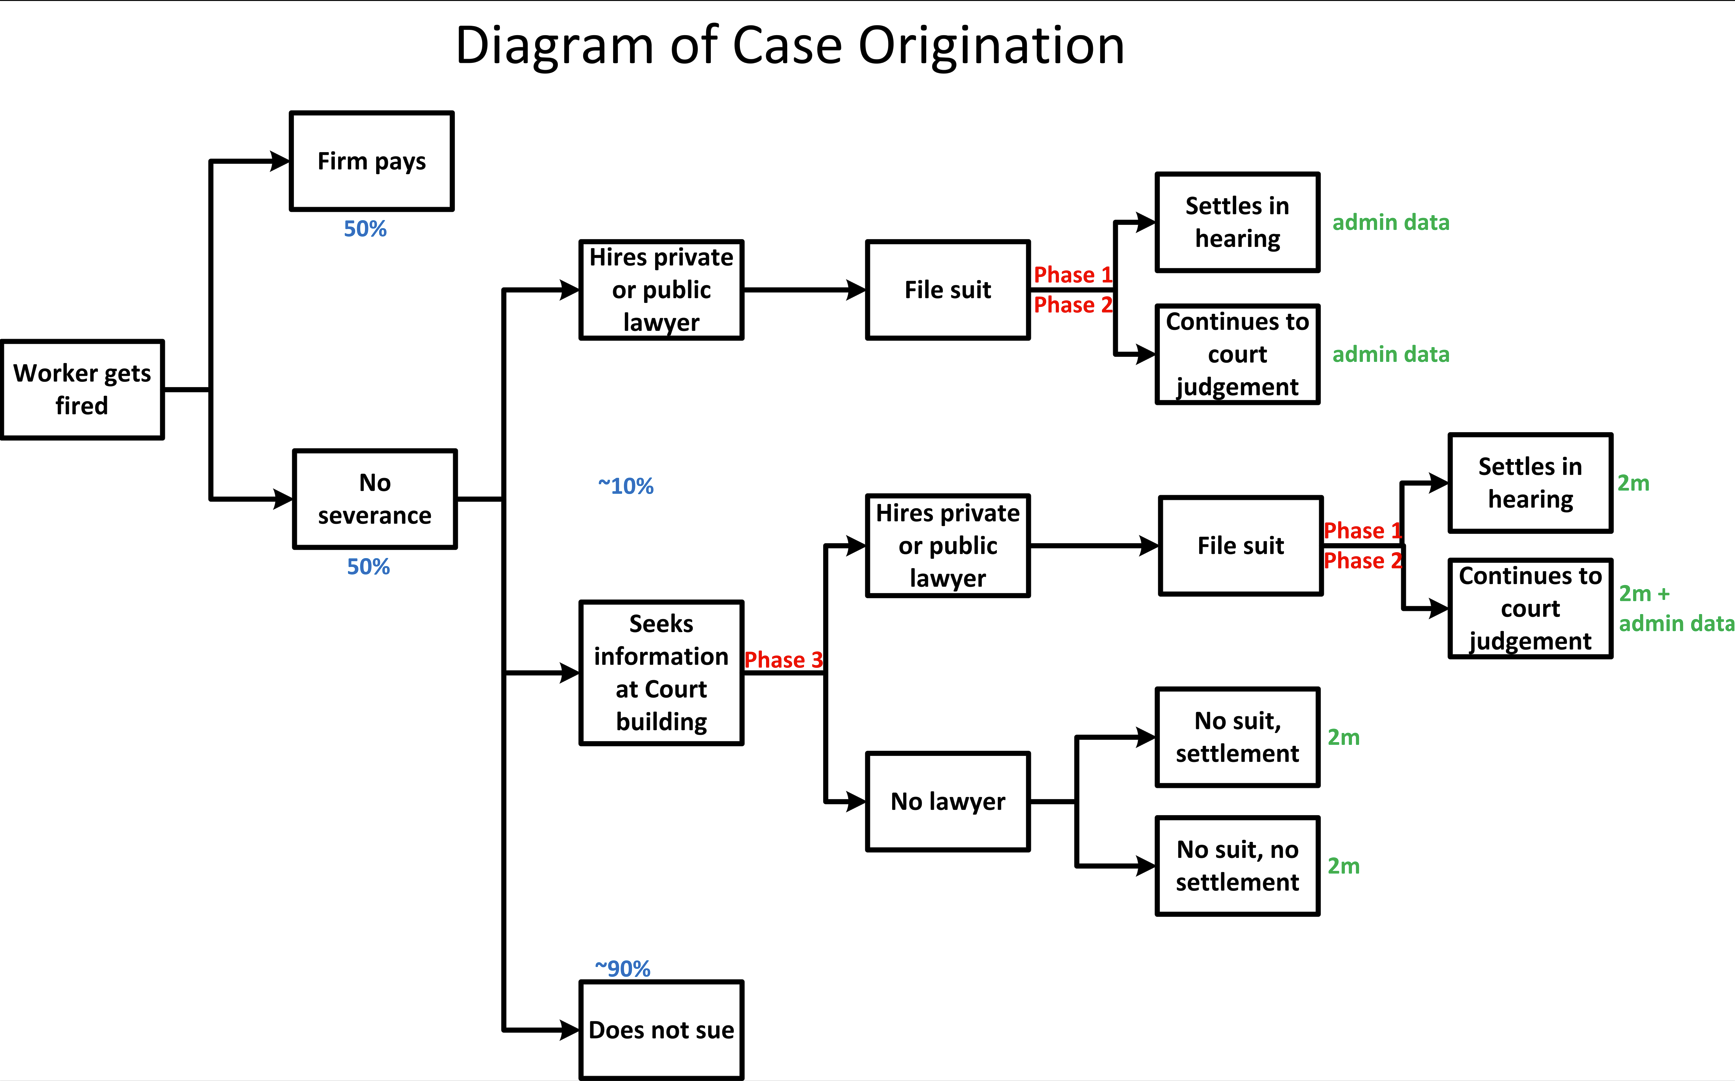
\includegraphics[width=0.9\textwidth]{paper/Figures/Diagram_Case_Origination_.png}
%         \end{center}

%     \label{stylized_representation}
% %\begin{figurenotes}
%     \scriptsize
% \textit{Notes:} This figure is a stylized representation of the process that casefiles follow in Mexico City's Labor Court.  
% %\end{figurenotes}    
% \end{figure}

\begin{figure}[!ht]
 \caption{Calculator Treatment Format (example) - Phase 2}
    \begin{center}
        \begin{subfigure}{0.49\textwidth}    
        \caption{Plaintiff}
             \centering
             
\includegraphics[width=1\textwidth]{calctreat_p2_act.pdf}
     \end{subfigure}
     \begin{subfigure}{0.49\textwidth}
     \caption{Defendant}
     \centering
         
\includegraphics[width=1\textwidth]{calctreat_p2_dem.pdf}
      \end{subfigure}
        \end{center}
           
    \label{calc_template_p2}
% \begin{figurenotes}
    \scriptsize
\textit{Notes:} The figure shows examples of the calculator treatment used in phase 2. The left panel format was given to the plaintiff / dismissed worker and the right panel format to the defendant. The calculator shows two numbers: first, for cases with similar characteristics that settled, the average amount obtained in settlement; second, each party's contingency in case they did not settle and proceeded to a judge's ruling. This is the likelihood of not obtaining any payment for the plaintiff and the recovery amount conditional on positive recovery for the defendant. As in phase 1, parties were told that this information comes from a statistical exercise based on completed historical cases, and that it gives average prediction based on variables of the initial lawsuit described in the calculator treatment.
% \end{figurenotes}
\end{figure}

\begin{figure}[!ht]
     \caption{Calculator Treatment Format (example) - Phase 3}
   \label{calc_template_p3}
   \begin{center}
       \scriptsize
        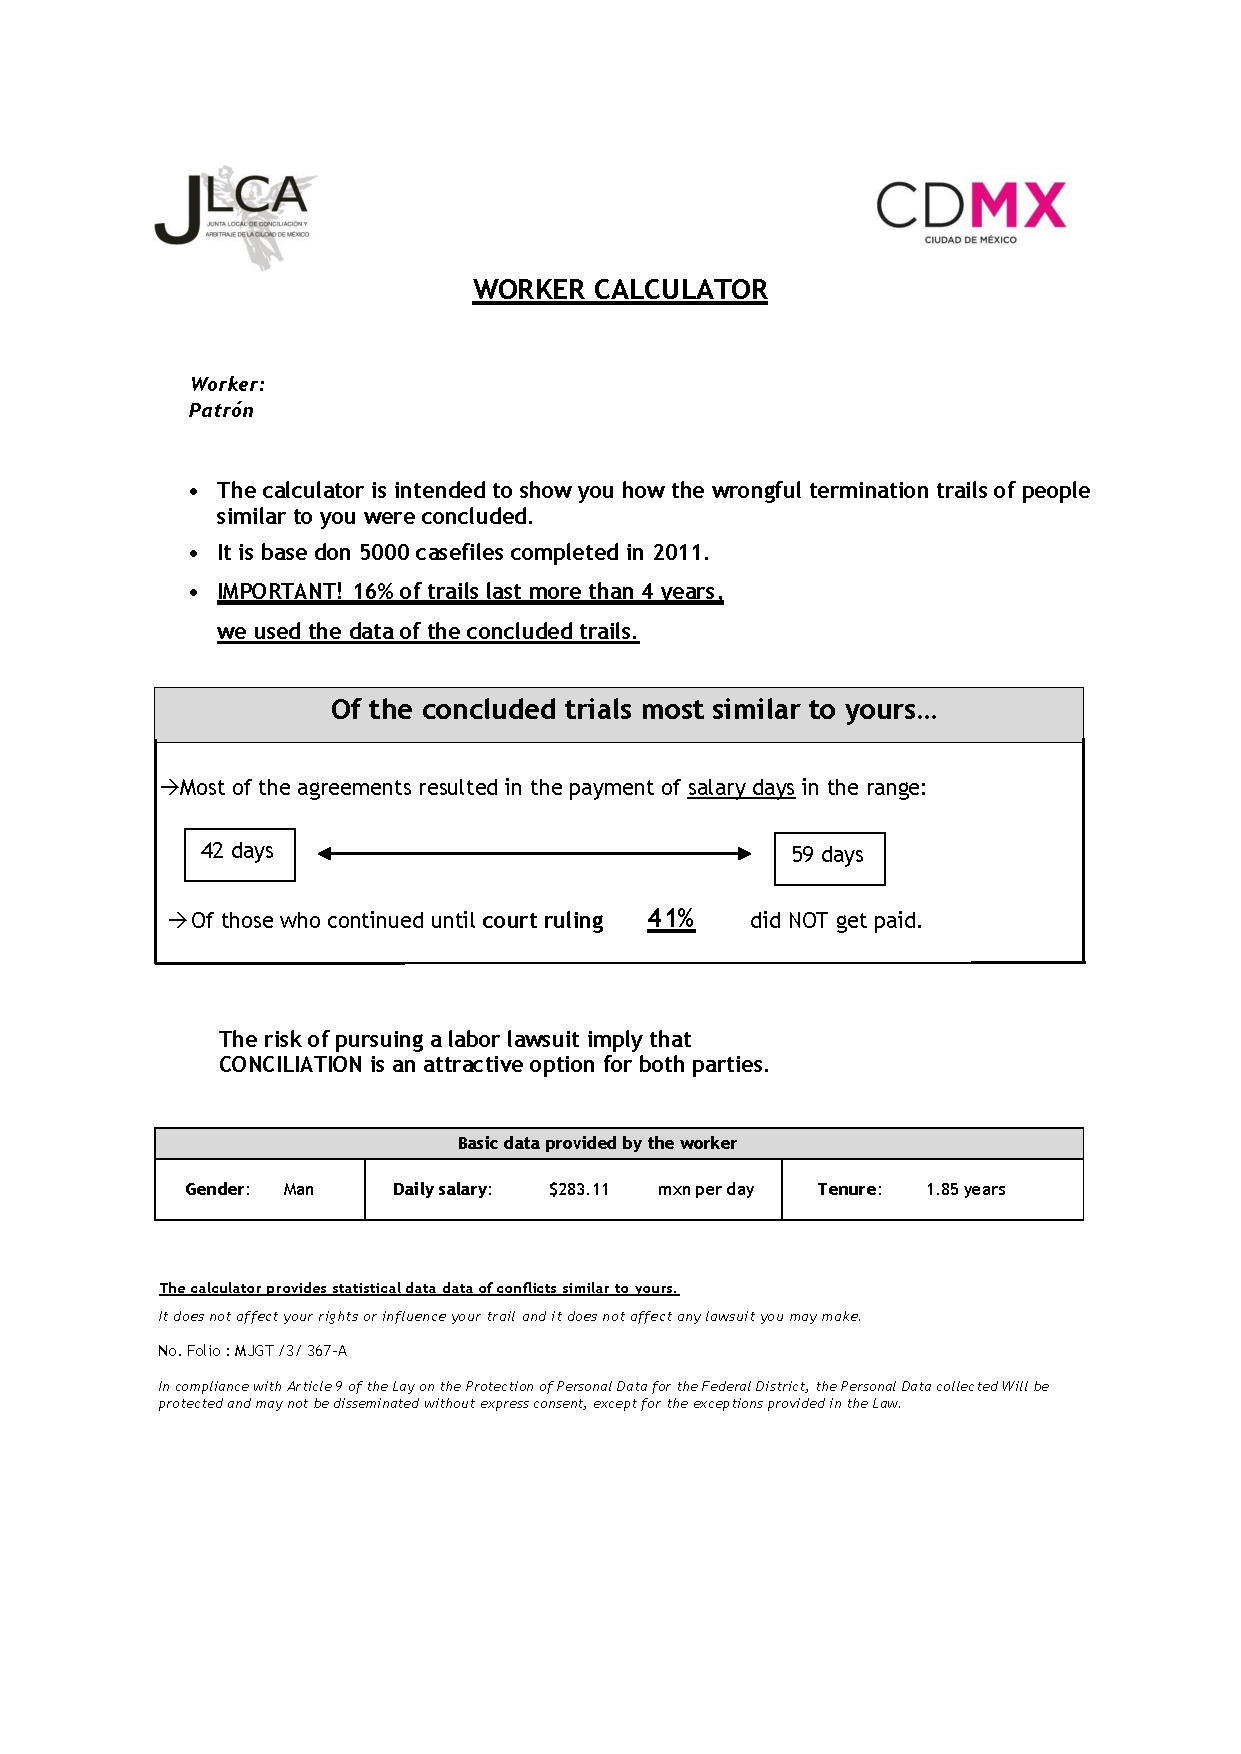
\includegraphics[width=0.5\textwidth]{paper/Figures/P3Treatments.pdf}
    \end{center}
           
 
% \begin{figurenotes}
    \scriptsize
\textit{Notes:} The figure shows an example of the calculator treatment provided to dismissed workers in phase 3. The calculator shows the inter-quartile range of settlement amounts expressed as the number of days paid and the percentage of cases continuing to court judgment where the plaintiff recovered nothing. The information provided is specific to the worker's characteristics. As in phases 1 and 2, parties were told that this information comes from a statistical exercise based on completed historical cases, and that it gives average prediction based on variables of the initial lawsuit described in the calculator treatment.
% \end{figurenotes}
\end{figure}
%\begin{figure}[!ht]
%    \caption{Prob plaintiff correctly knows what is in the lawsuit}
%    \label{knowledge_private}
%   \begin{center}
%        
\includegraphics[width=0.8\textwidth]{knowledge_law_graph.pdf}
%        \end{center}
%        {\scriptsize \textit{Notes:} We regress a dummy variable indicating the plaintiff correctly answered a question about the contents of her case against a variable indicating the plaintiff is represented by a public lawyer. Each pair of bars shows the coefficient from the regression on the case characteristic shown in the label on the $x$ axis. In each pair, the left-hand bar is the coefficient from a regression without any control variables and the right-hand bar is the coefficient from a regression including the six basic case controls. The whisker lines represent the 95 \% confidence limits. The data indicate that clients of public lawyers are significantly more knowledgeable about the contents of their cases than are clients of private lawyers for four of the five case characteristics. 
        
        %\textit{Do File: } \texttt{knowledge\_law\_graph.do}
%        }
%\end{figure}

\begin{figure}[!ht]
\caption{Distribution of Amount Collected, by Type of Lawyer}
    \begin{center}
        
\includegraphics[width=0.9\textwidth]{cdf_pdf_value_claims.pdf}
        \end{center}
    \label{cdf_value_claims}
% \begin{figurenotes}
    \scriptsize
\textit{Notes:} This Figure uses the historical data to show cumulative distributions and densities of the amount received in the historical data. It uses all casefiles endings (court ruling, settlements, drop and expiry). Amounts on the x-axis are in thousand pesos and brought to present value to the time of suing, with a monthly interest rate of 3.43. Since we care about what the worker actually receives, when they use a private lawyer we subtract a 30\% of the recovery and the initial filing feel. The graph shows outcomes for three different initial fees (indicated in the legend): MXN\$2,000 pesos, MXN\$1,000 pesos, and MXN\$500 pesos. The modal fee in the survey data is MXN\$2,000 pesos. To the left of the vertical line at zero the worker loses money (from the initial fee). The figure indicates that there are a large fraction of cases where the worker has a negative net recovery.
    %{\scriptsize \textit{Do file: } \texttt{Fig2_cdf_value_claims_rep.do}}
% \end{figurenotes}    
\end{figure}

\begin{figure}[!ht]
    \caption{Subjective expectation minus prediction - Phase 1}
    \label{Figure_overconfidence_exp}
    \begin{center}
    \begin{subfigure}{0.45\textwidth}
        \caption{Employee}
        \centering
        
\includegraphics[width=\linewidth]{diff_amt_e.pdf}
    \end{subfigure}
    \begin{subfigure}{0.45\textwidth}
        \centering
        
\includegraphics[width=\linewidth]{diff_prob_e.pdf}
        \end{subfigure}
        \begin{subfigure}{0.45\textwidth}
            \caption{Employee's Lawyer}
            \centering
            
\includegraphics[width=\linewidth]{diff_amt_el.pdf}
    \end{subfigure}
    \begin{subfigure}{0.45\textwidth}
        \centering
        
\includegraphics[width=\linewidth]{diff_prob_el.pdf}
    \end{subfigure}
    \begin{subfigure}{0.45\textwidth}
        \caption{Firm's Lawyer}
        \centering
        
\includegraphics[width=\linewidth]{diff_amt_fl.pdf}
        \end{subfigure}
        \begin{subfigure}{0.45\textwidth}
            \centering
            
\includegraphics[width=\linewidth]{diff_prob_fl.pdf}   
    \end{subfigure}        
    \end{center}
      \scriptsize \textit{Notes:} Difference in thousand pesos for amounts (panel on left) and percentage points for probabilities (panel on right) from what the subject expects vs. what our models predict. Note how, for Employee and employee lawyer, the distribution for amounts is much more skewed to the right than for firm lawyers. This is only natural, since the former are thinking about expected wins and the latter about expected losses. 
    %   \scriptsize{ \textit{Do file: }  \texttt{oc\_comparison\_B.do}}
\end{figure}

\begin{figure}[!ht]
    \caption{Settlement Amount vs. Calculator}
        \label{RatioCalculator_Settlements}
    \begin{center}
        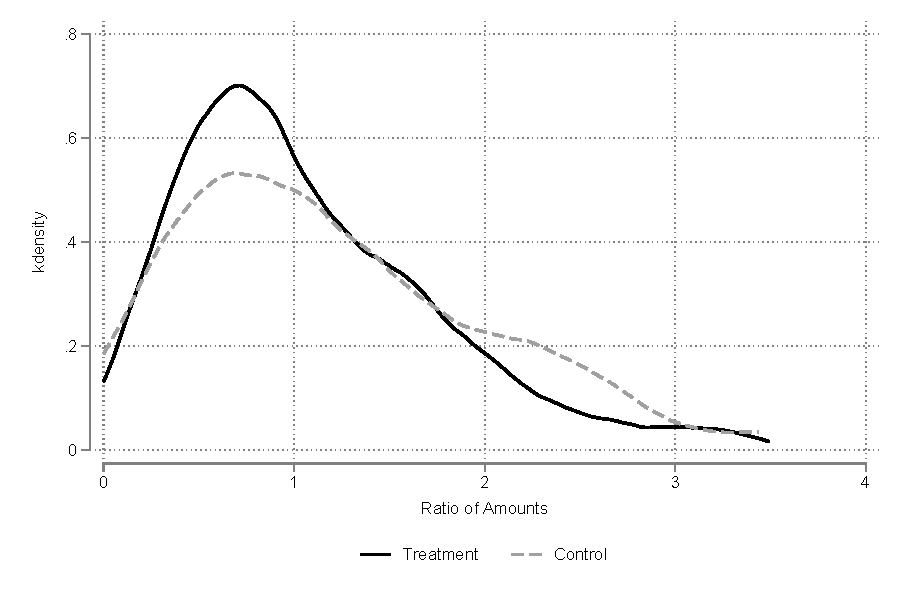
\includegraphics[width=0.6\textwidth]{paper/Figures/kdensityRatio.pdf}
         \end{center}
              \scriptsize
             \textit{Notes:} This figure presents the distribution of actual settlement amount over the calculator prediction. Data are truncated at the 99th percentile to compress the scale.
        %\textit{Do file: } \texttt{ratioGananciaConvenio.do}   
\end{figure}

\begin{figure}[!ht]
    \caption{Outcomes when Plaintiff was Present, by Treatment}
    \label{OutcomesByTreatment}
       \begin{center}
   \begin{subfigure}{0.45\textwidth}
        \caption{Phase 1}
        \centering
        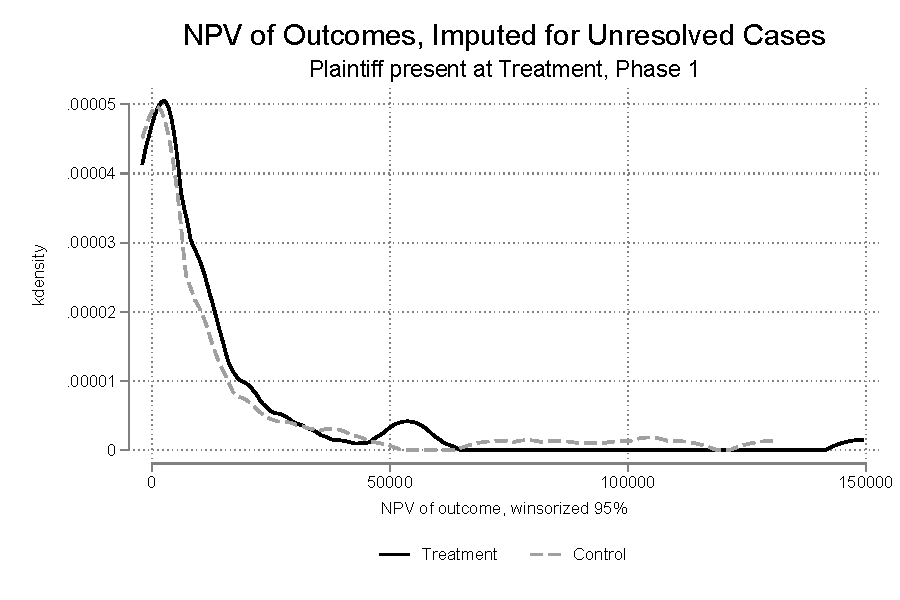
\includegraphics[width=\linewidth]{paper/Figures/OutcomesByTreatment_P1.pdf}
    \end{subfigure}
   \begin{subfigure}{0.45\textwidth}
        \caption{Phase 2}
        \centering
        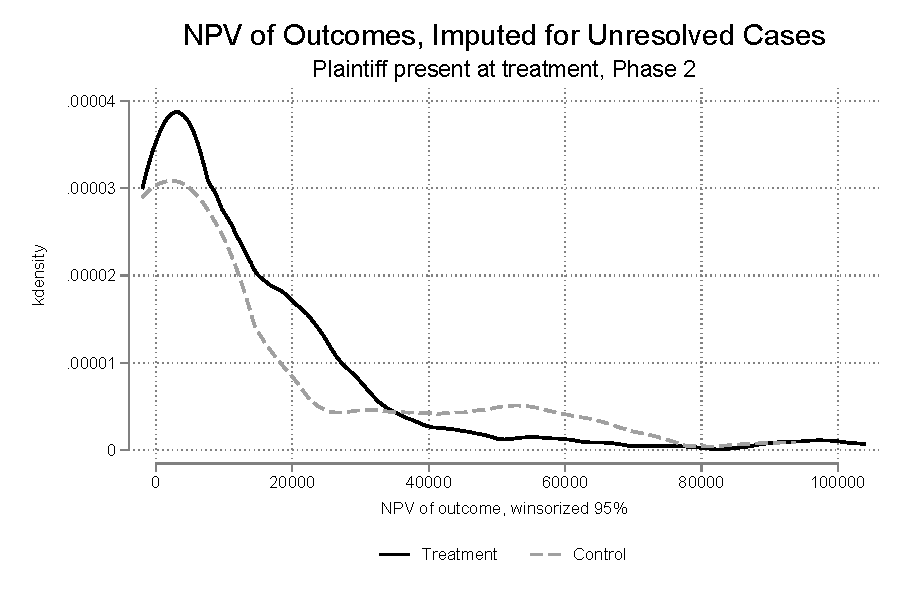
\includegraphics[width=\linewidth]{paper/Figures/OutcomesByTreatment_P2.pdf}
    \end{subfigure}
 
   
   \end{center}
      \scriptsize \textit{Notes:} This figure shows the kernel density of the NPV of the amount awarded by treatment and phase of the intervention. NPV is discounted at an annual rate of 50 percent and the value of unresolved cases is imputed from the calculator prediction for outcome by court judgment. Data are winsorized at the 95th percentile.
    %   \scriptsize{ \textit{Do file: }  \texttt{followup2020_newSpecificationitt_both}}
\end{figure}

\begin{figure}[!ht]
    \caption{Calculator Predictions for Plaintiff Court Judgment, By Phase}
    \label{Unresolved_Court_ByPhase}
       \begin{center}
   \begin{subfigure}{0.45\textwidth}
        \caption{Phase 1}
        \centering
        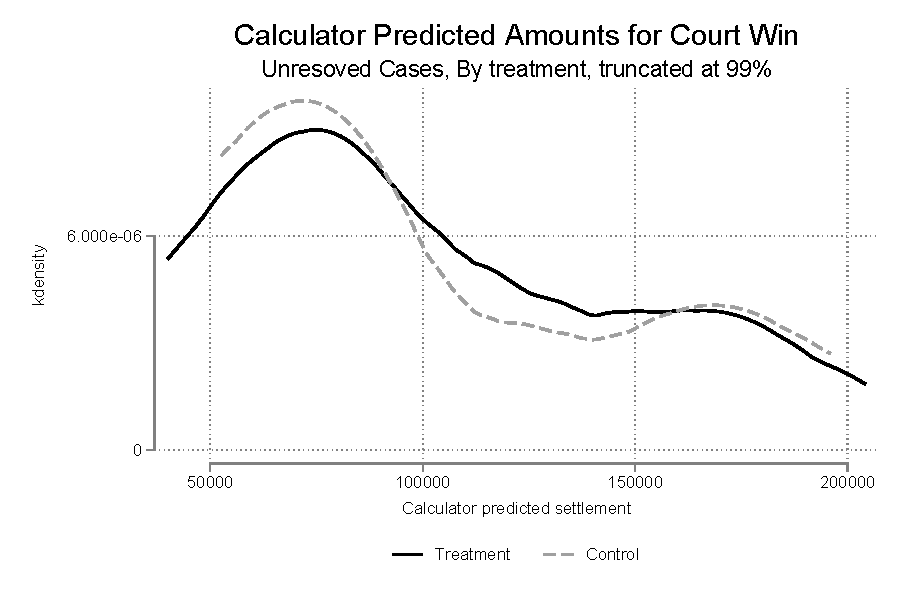
\includegraphics[width=\linewidth]{paper/Figures/Calculator_CourtWin_Unresolved_P1.pdf}
    \end{subfigure}
   \begin{subfigure}{0.45\textwidth}
        \caption{Phase 2}
        \centering
        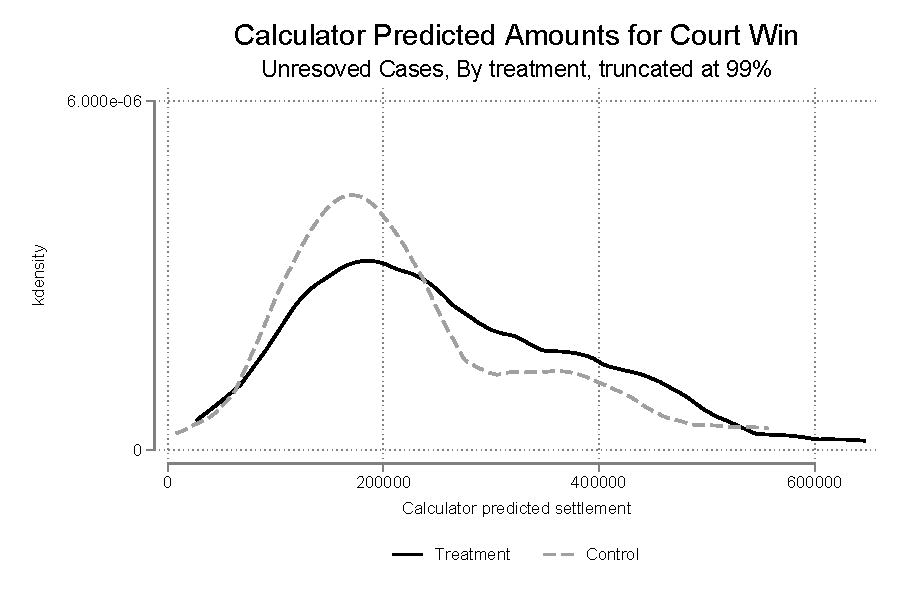
\includegraphics[width=\linewidth]{paper/Figures/Calculator_CourtWin_Unresolved_P2.pdf}
    \end{subfigure}
 
   
   \end{center}
      \scriptsize \textit{Notes:} This figure presents the calculator prediction for amount recovered conditional on the plaintiff winning a court judgment, for treatment and control cases that were unresolved as of 2020. The cases in phase 1 and phase 2 are shown separately.  Data are truncated at the 99th percentile to compress the scale.
    %   \scriptsize{ \textit{Do file: }  \texttt{casevaluekdensitiesdo.do}}
\end{figure}

\begin{figure}[!ht]
    \caption{Information handed out in placebo test}
        \label{placebo_leaflet}
    \begin{center}
        
\includegraphics[width=0.4\textwidth]{placebo_information.pdf}
         \end{center}
              \scriptsize
             \textit{Notes:} This is the information brochure handed out to subjects in the placebo test. Essentially, it is a reminder of the existence of the conciliation process, which is free, confidential and unbiased.
\end{figure}

\begin{figure}[!ht]
    \caption{Discount rate for Phase 1 and MxFLS}
        \label{mxfls_comp}
    \begin{center}
        
\includegraphics[width=0.6\textwidth]{discount_rate_tp_comp.pdf}
         \end{center}
              \scriptsize
             \textit{Notes:} Comparison of discount rates for Phase 1 data and survey data from the MxFLS (Mexican Family Life Survey-  a longitudinal survey in Mexico that follows individuals across rounds). In both surveys individuals are asked whether they would choose to receive \$1,000 dollars today or an array of different values in the future (\$1,200, \$1,500, \$2,000 or \$3,000 dollars). The monthly discount rate is calculated by dividing the \$1,000 dollars over the choice made by individuals.   
        %\textit{Do file: } \texttt{discount\_rate\_ph1\_mxfls.do}                   
\end{figure}

%\begin{figure}[!ht]
%    \caption{Propensity score overlap}
%        \label{ps_overlap}
%    \begin{center}
%        
\includegraphics[width=0.6\textwidth]{ps_overlap.pdf}
%         \end{center}
%              \scriptsize
%             \textit{Notes:} The graph shows the overlap between the propensity scores after the trimming procedure suggested by \cite{CHIM_2009} and \cite{Imbens2015} when performing the analysis for table \ref{match_table}.
    %\textit{Do file: } \texttt{settlement\_conciliator\_matching.do}          
%\end{figure}



%\begin{figure}[!ht]
%    \caption{Discount rate against welfare effects}
%        \label{atematch_inrate}
%    \begin{center}
%        
\includegraphics[width=0.6\textwidth]{atematch_intrate.pdf}
%         \end{center}
%              \scriptsize
%             \textit{Notes:} The graph shows the ATE effect of Table \ref{match_table} column (4), when using different discounting annual interest rates. 
    %\textit{Do file: } \texttt{settlement\_conciliator\_matching\_interest\_rate.do}          
%\end{figure}

%%%%%%%%%%%%%%%%%% EXPERIMENT FIGURES




